% Options for packages loaded elsewhere
\PassOptionsToPackage{unicode}{hyperref}
\PassOptionsToPackage{hyphens}{url}
%
\documentclass[
]{book}
\usepackage{lmodern}
\usepackage{amsmath}
\usepackage{ifxetex,ifluatex}
\ifnum 0\ifxetex 1\fi\ifluatex 1\fi=0 % if pdftex
  \usepackage[T1]{fontenc}
  \usepackage[utf8]{inputenc}
  \usepackage{textcomp} % provide euro and other symbols
  \usepackage{amssymb}
\else % if luatex or xetex
  \usepackage{unicode-math}
  \defaultfontfeatures{Scale=MatchLowercase}
  \defaultfontfeatures[\rmfamily]{Ligatures=TeX,Scale=1}
\fi
% Use upquote if available, for straight quotes in verbatim environments
\IfFileExists{upquote.sty}{\usepackage{upquote}}{}
\IfFileExists{microtype.sty}{% use microtype if available
  \usepackage[]{microtype}
  \UseMicrotypeSet[protrusion]{basicmath} % disable protrusion for tt fonts
}{}
\makeatletter
\@ifundefined{KOMAClassName}{% if non-KOMA class
  \IfFileExists{parskip.sty}{%
    \usepackage{parskip}
  }{% else
    \setlength{\parindent}{0pt}
    \setlength{\parskip}{6pt plus 2pt minus 1pt}}
}{% if KOMA class
  \KOMAoptions{parskip=half}}
\makeatother
\usepackage{xcolor}
\IfFileExists{xurl.sty}{\usepackage{xurl}}{} % add URL line breaks if available
\IfFileExists{bookmark.sty}{\usepackage{bookmark}}{\usepackage{hyperref}}
\hypersetup{
  pdftitle={Supplement to MA206 Probability and Statistics},
  pdfauthor={Authors TBD},
  hidelinks,
  pdfcreator={LaTeX via pandoc}}
\urlstyle{same} % disable monospaced font for URLs
\usepackage{longtable,booktabs}
\usepackage{calc} % for calculating minipage widths
% Correct order of tables after \paragraph or \subparagraph
\usepackage{etoolbox}
\makeatletter
\patchcmd\longtable{\par}{\if@noskipsec\mbox{}\fi\par}{}{}
\makeatother
% Allow footnotes in longtable head/foot
\IfFileExists{footnotehyper.sty}{\usepackage{footnotehyper}}{\usepackage{footnote}}
\makesavenoteenv{longtable}
\usepackage{graphicx}
\makeatletter
\def\maxwidth{\ifdim\Gin@nat@width>\linewidth\linewidth\else\Gin@nat@width\fi}
\def\maxheight{\ifdim\Gin@nat@height>\textheight\textheight\else\Gin@nat@height\fi}
\makeatother
% Scale images if necessary, so that they will not overflow the page
% margins by default, and it is still possible to overwrite the defaults
% using explicit options in \includegraphics[width, height, ...]{}
\setkeys{Gin}{width=\maxwidth,height=\maxheight,keepaspectratio}
% Set default figure placement to htbp
\makeatletter
\def\fps@figure{htbp}
\makeatother
\setlength{\emergencystretch}{3em} % prevent overfull lines
\providecommand{\tightlist}{%
  \setlength{\itemsep}{0pt}\setlength{\parskip}{0pt}}
\setcounter{secnumdepth}{5}
\usepackage{booktabs}
\ifluatex
  \usepackage{selnolig}  % disable illegal ligatures
\fi
\usepackage[]{natbib}
\bibliographystyle{apalike}

\title{Supplement to MA206 Probability and Statistics}
\author{Authors TBD}
\date{2021-03-05}

\begin{document}
\maketitle

{
\setcounter{tocdepth}{1}
\tableofcontents
}
\hypertarget{motivation}{%
\chapter{Motivation}\label{motivation}}

\hypertarget{goals-of-statistical-analyses-describe-predict-cause-and-effect}{%
\section{Goals of statistical analyses (describe, predict, cause-and-effect)}\label{goals-of-statistical-analyses-describe-predict-cause-and-effect}}

\hypertarget{why-multivariable-methods}{%
\section{Why multivariable methods?}\label{why-multivariable-methods}}

\hypertarget{why-multiple-regression}{%
\section{Why multiple regression?}\label{why-multiple-regression}}

\hypertarget{causality}{%
\chapter{Causality}\label{causality}}

\hypertarget{what-does-it-mean-for-one-thing-to-cause-another}{%
\section{What does it mean for one thing to cause another}\label{what-does-it-mean-for-one-thing-to-cause-another}}

\hypertarget{randomized-controlled-experiments}{%
\section{Randomized controlled experiments}\label{randomized-controlled-experiments}}

\hypertarget{observational-studies}{%
\section{Observational Studies}\label{observational-studies}}

\hypertarget{confounding}{%
\section{Confounding}\label{confounding}}

\hypertarget{causal-diagrams}{%
\section{Causal Diagrams}\label{causal-diagrams}}

\hypertarget{categorical}{%
\chapter{Quantitative explanatory variable with categorical confounding variable}\label{categorical}}

Introduce multiple regression by adding a categorical confounding variable

Explanatory (\(X\)) - quantitative

Response (\(Y\)) - quantitative

Confounding (\(C\)) - categorical

\hypertarget{unadjusted-effect-of-x-on-y}{%
\section{\texorpdfstring{Unadjusted effect of \(X\) on \(Y\)}{Unadjusted effect of X on Y}}\label{unadjusted-effect-of-x-on-y}}

short review of simple regression

\hypertarget{effect-of-x-and-y-adjusting-for-c.}{%
\section{\texorpdfstring{Effect of \(X\) and \(Y\) adjusting for \(C\).}{Effect of X and Y adjusting for C.}}\label{effect-of-x-and-y-adjusting-for-c.}}

\hypertarget{assessing-model-adequacy}{%
\section{Assessing model adequacy}\label{assessing-model-adequacy}}

\hypertarget{interactions}{%
\chapter{Interactions}\label{interactions}}

Extend the example in the last chapter\ldots introduce in terms of effect modification. We have a new research question, ``does the affect of \(X\) on \(Y\) change based on another variable of interest?''

\hypertarget{activity}{%
\chapter{Activity}\label{activity}}

\emph{Title}: The Indoor Obstacle Course Test (IOCT)

\emph{Topics}\}*: Confounding, Causal Diagrams, Simple Linear Regression, Confidence Intervals

\emph{Background}: Cadets at West Point must pass the \href{https://www.youtube.com/watch?v=94tPO0fGtJo\&t=77s}{Indoor Obstacle Course Test} (IOCT) to graduate. The IOCT begins with a series of floor and climbing obstacles and ends with several laps around an indoor track. It is an exhausting test of endurance and strength. In addition to being a graduation requirement, cadets receive a letter grade that is factored into their class rank.

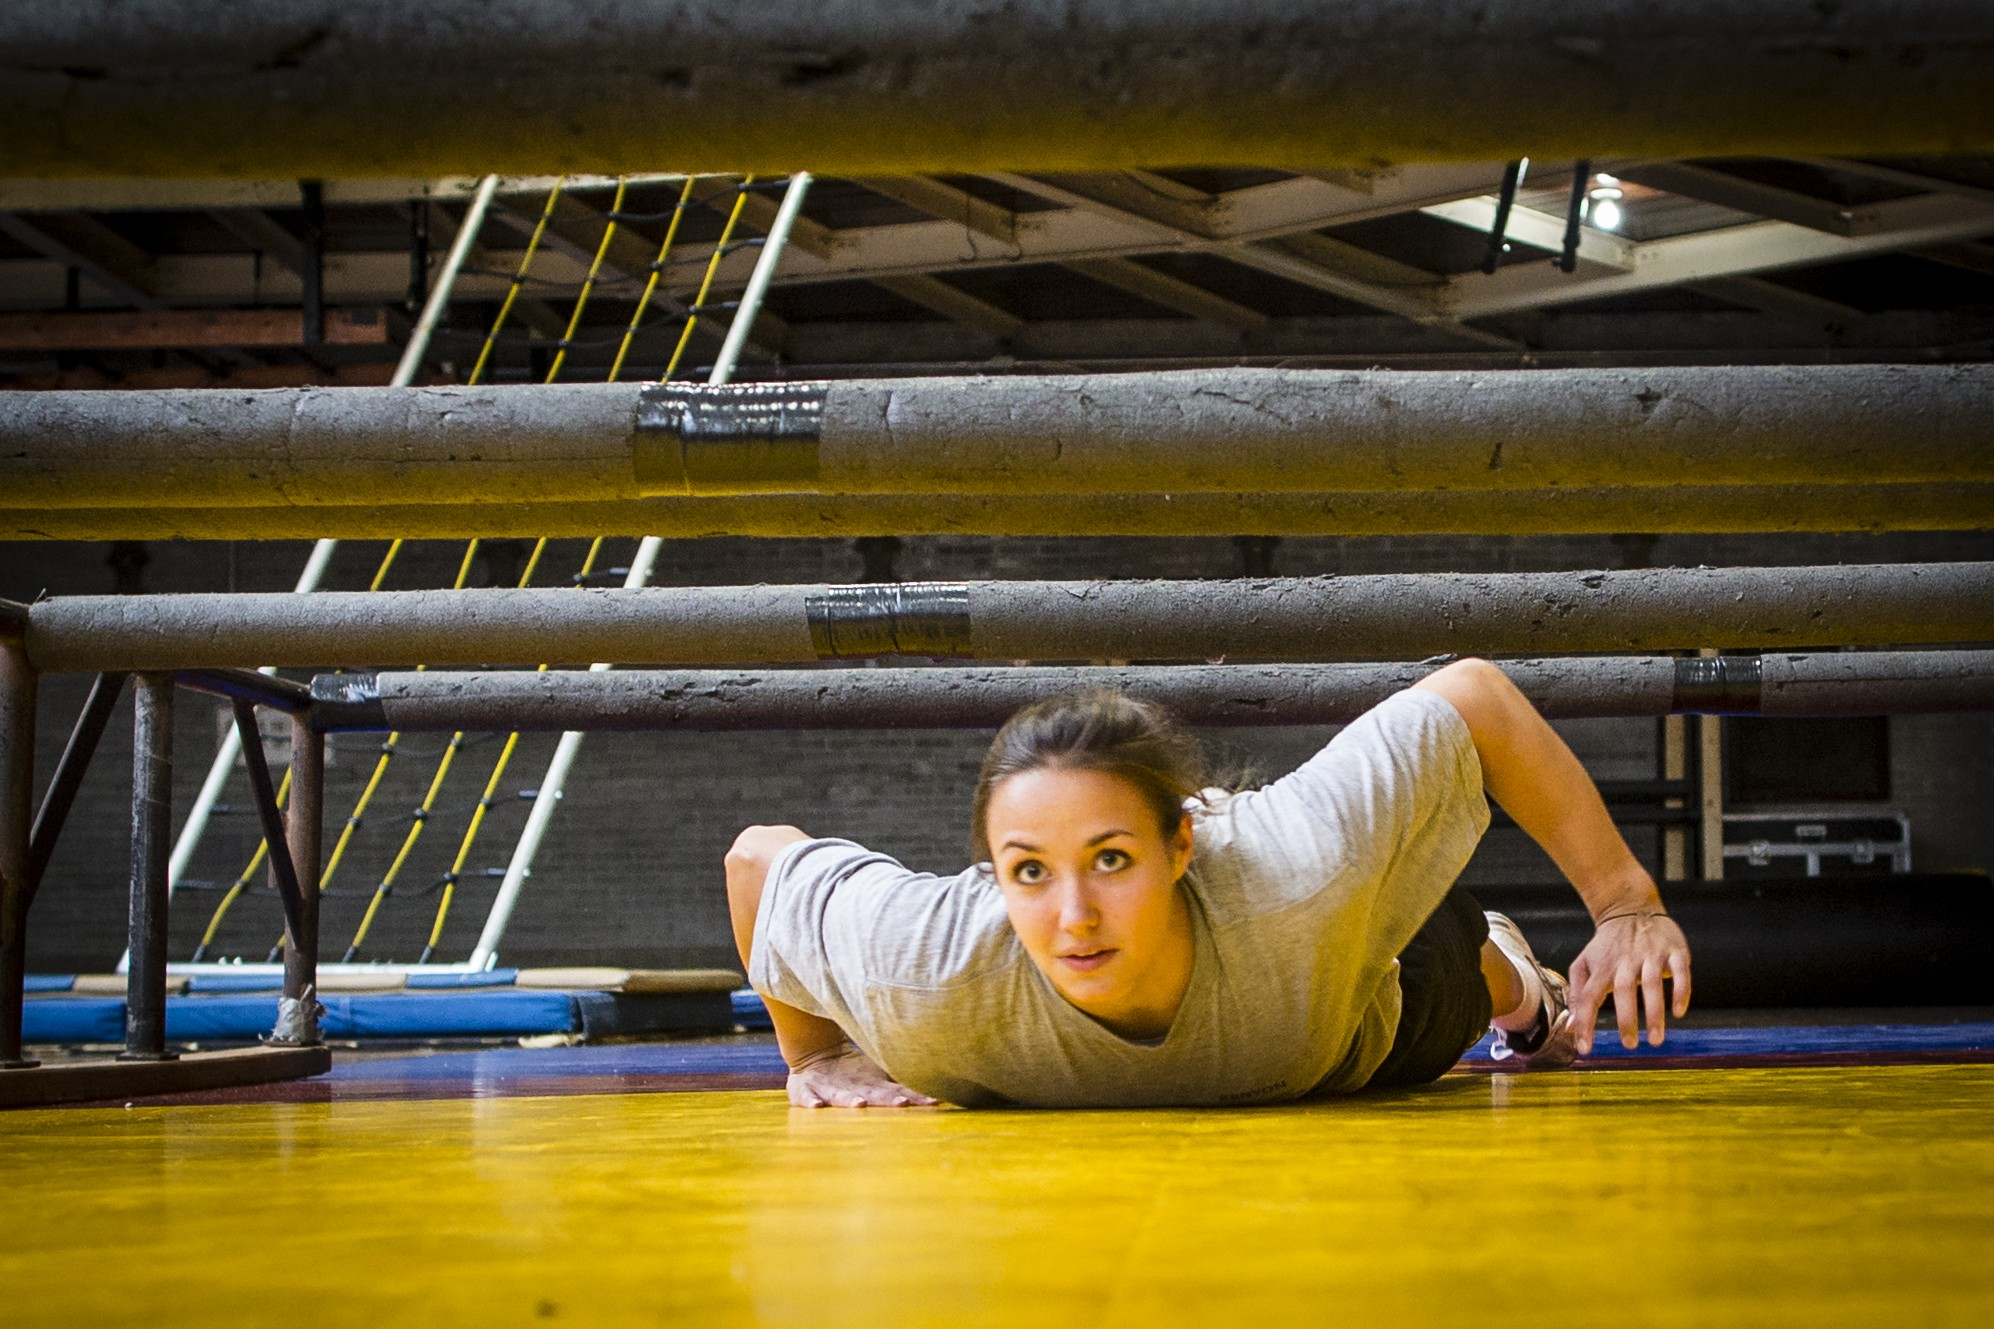
\includegraphics[width=0.5\textwidth,height=\textheight]{./images/crawlObstacle.jpg} 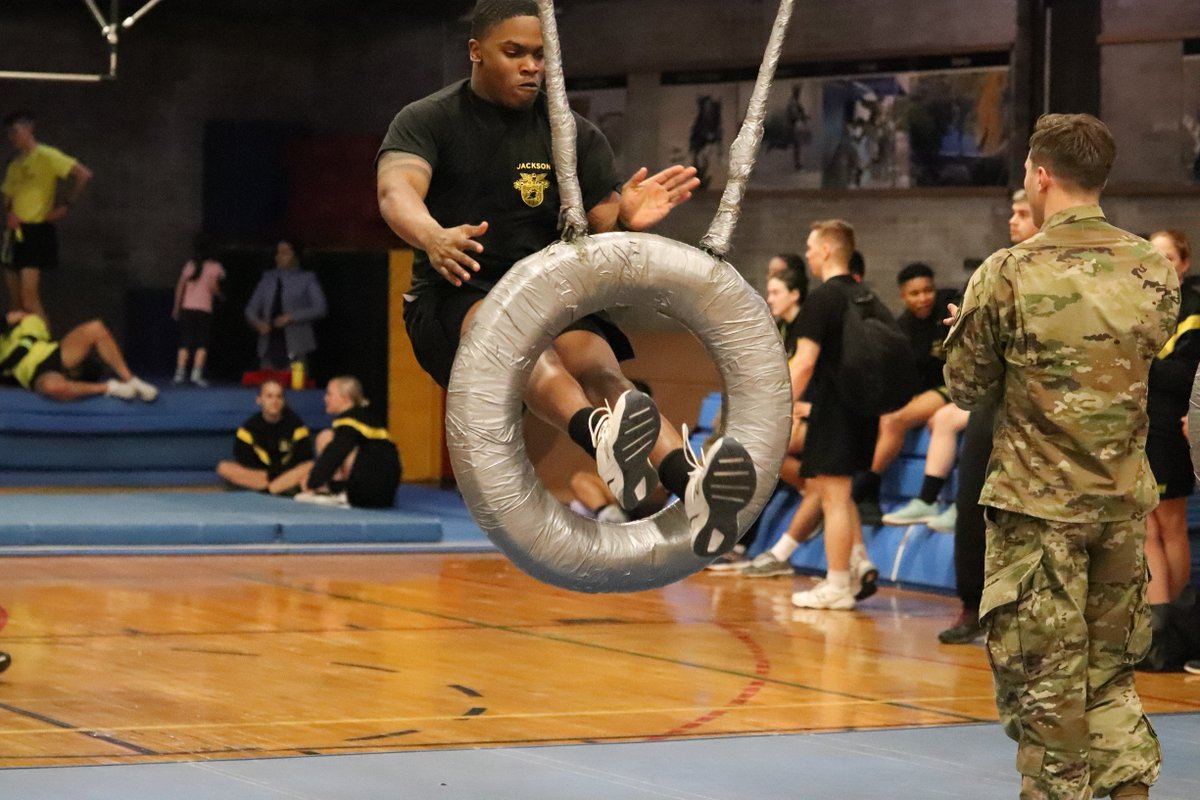
\includegraphics[width=0.5\textwidth,height=\textheight]{./images/tireObstacle.jpg}

Shorter cadets often argue they are at a disadvantage on the obstacle course. Many obstacles appear to favor taller cadets because they are easier to reach. In this study, we will investigate the effect of height on IOCT times.

\begin{enumerate}
\def\labelenumi{\arabic{enumi}.}
\tightlist
\item
  \href{https://www.youtube.com/watch?v=94tPO0fGtJo\&t=77s}{Watch the video of Cadet Madaline Kenyon running the IOCT}. In your opinion, do some obstacles favor taller cadets? Explain.
\end{enumerate}

\vspace{1in}

The file \texttt{obstacle\_course.csv} contains height (inches), IOCT times (seconds), biological sex (M/F), and whether the cadet played an intercollegiate sport for a sample of 384 cadets who ran the IOCT course in the last five years.

\begin{enumerate}
\def\labelenumi{\arabic{enumi}.}
\setcounter{enumi}{1}
\tightlist
\item
  What is the explanatory variable in this study? Classify the variable as quantitative or categorical.
\end{enumerate}

\vspace{0.25in}

\begin{enumerate}
\def\labelenumi{\arabic{enumi}.}
\setcounter{enumi}{2}
\tightlist
\item
  What is the response variable in this study? Classify the variable as quantitative or categorical.
\end{enumerate}

\vspace{0.25in}

\begin{enumerate}
\def\labelenumi{\arabic{enumi}.}
\setcounter{enumi}{3}
\tightlist
\item
  Is this study an observational study or a randomized experiment? Explain.
\end{enumerate}

\vspace{1in}

\newpage

Figure 1 depicts IOCT times in seconds versus height in inches. Table 1 contains information from the linear regression model.

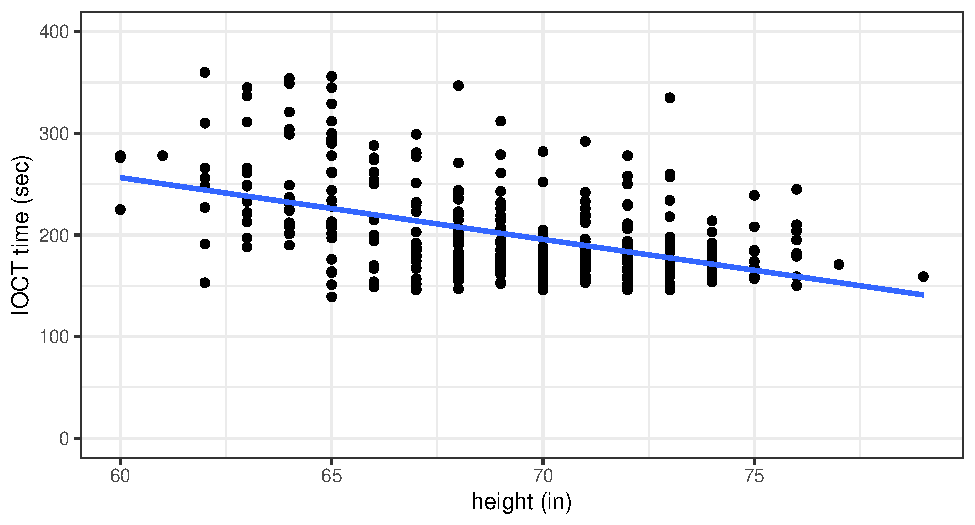
\includegraphics{MA206supplement_files/figure-latex/unnamed-chunk-2-1.pdf}

\begin{table}

\caption{\label{tab:unnamed-chunk-2}Linear regression output for IOCT times and height.}
\centering
\begin{tabular}[t]{l|r|r|r|r}
\hline
term & estimate & std.error & statistic & p.value\\
\hline
(Intercept) & 621.00 & 39.98 & 15.53 & 0\\
\hline
height & -6.08 & 0.58 & -10.52 & 0\\
\hline
\end{tabular}
\end{table}

\begin{enumerate}
\def\labelenumi{\arabic{enumi}.}
\setcounter{enumi}{4}
\item
  Interpret the estimate of the height coefficient in Table 1.

  \vspace{1in}
\item
  Calculate and interpret a 95\% confidence interval for the slope coefficient.
\end{enumerate}

\vspace{1in}

\newpage

\begin{enumerate}
\def\labelenumi{\arabic{enumi}.}
\setcounter{enumi}{6}
\tightlist
\item
  The \(p\)-value for height in Table 1 indicates there is strong evidence of an association between height and IOCT time. Taller cadets tend to do better on the IOCT. Some people would say the result is \emph{statistically significant}. However, statistical significance and practical signifigance are different. \href{https://en.wikipedia.org/wiki/Indoor_Obstacle_Course_Test}{Review the grade scale for the IOCT.} In your opinion, does the observed association have practical significance? Explain.
\end{enumerate}

\vspace{1in}

\begin{enumerate}
\def\labelenumi{\arabic{enumi}.}
\setcounter{enumi}{7}
\tightlist
\item
  A shorter cadet argues Figure 1 shows evidence the IOCT is unfair based on height. Do you agree or disagree? Explain.
\end{enumerate}

\vspace{1in}

\begin{enumerate}
\def\labelenumi{\arabic{enumi}.}
\setcounter{enumi}{8}
\tightlist
\item
  Briefly explain the difference between these two conclusions.
\end{enumerate}

\begin{itemize}
\item
  \emph{Height is associated with faster IOCT times.}
\item
  \emph{Height causes faster IOCT times.}
\end{itemize}

\vspace{1in}

\begin{enumerate}
\def\labelenumi{\arabic{enumi}.}
\setcounter{enumi}{9}
\tightlist
\item
  Based on the analysis presented thus far, is it possible to distinguish between these two explanations? Explain.
\end{enumerate}

\vspace{1in}

\begin{enumerate}
\def\labelenumi{\arabic{enumi}.}
\setcounter{enumi}{10}
\tightlist
\item
  Draw a causal diagram depicting the relationship between height, IOCT time, and sex. Explain your decisions to include/exclude arrows in the diagram.
\end{enumerate}

\vspace{1in}

\begin{enumerate}
\def\labelenumi{\arabic{enumi}.}
\setcounter{enumi}{11}
\tightlist
\item
  Based on your diagram, identify the confounding variable.
\end{enumerate}

\vspace{0.5in}

Below are boxplots of height in inches and IOCT times in seconds by sex.

\begin{figure}
\centering
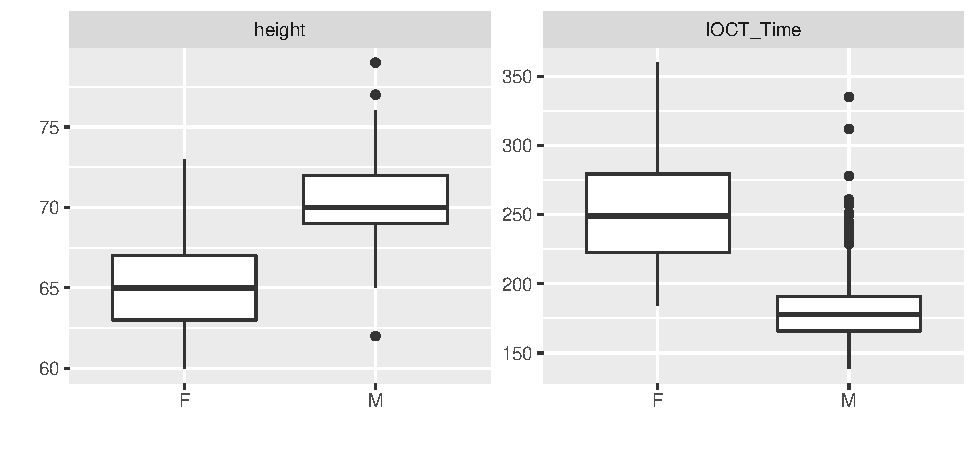
\includegraphics{MA206supplement_files/figure-latex/unnamed-chunk-3-1.pdf}
\caption{\label{fig:unnamed-chunk-3}Height (inches) and IOCT time (seconds) by sex.}
\end{figure}

\begin{enumerate}
\def\labelenumi{\arabic{enumi}.}
\setcounter{enumi}{12}
\tightlist
\item
  Based on Figure 2, is the estimate of the effect of height on IOCT time in Table 1 confounded by sex? If so, is the effect of height smaller or larger than that reported in Table 1? Explain.
\end{enumerate}

\vspace{1in}

\newpage

Figure 3 depicts the association between IOCT time and height by sex. Tables 2 and 3 depict regression results for female and male cadets, respectively.

\begin{figure}
\centering
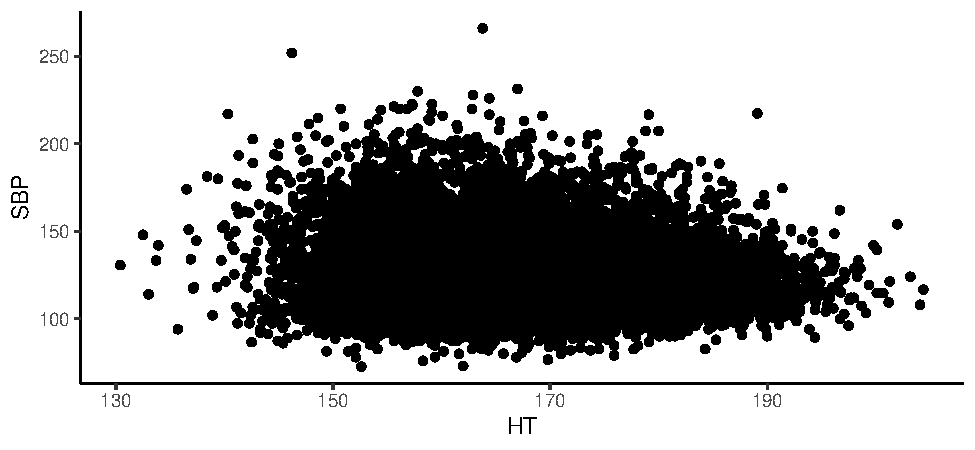
\includegraphics{MA206supplement_files/figure-latex/unnamed-chunk-4-1.pdf}
\caption{\label{fig:unnamed-chunk-4}Indoor Obstacle Course Test (IOCT) times versus height by sex (n = 384).}
\end{figure}

\begin{table}

\caption{\label{tab:unnamed-chunk-5}Regression results for female cadets.}
\centering
\begin{tabular}[t]{l|r|r|r|r}
\hline
term & estimate & std.error & statistic & p.value\\
\hline
(Intercept) & 335.76 & 107.44 & 3.12 & 0.00\\
\hline
height & -1.24 & 1.64 & -0.76 & 0.45\\
\hline
\end{tabular}
\end{table}

\begin{table}

\caption{\label{tab:unnamed-chunk-5}Regression results for male cadets.}
\centering
\begin{tabular}[t]{l|r|r|r|r}
\hline
term & estimate & std.error & statistic & p.value\\
\hline
(Intercept) & 175.61 & 40.92 & 4.29 & 0.00\\
\hline
height & 0.09 & 0.58 & 0.15 & 0.88\\
\hline
\end{tabular}
\end{table}

\begin{enumerate}
\def\labelenumi{\arabic{enumi}.}
\setcounter{enumi}{13}
\tightlist
\item
  Based on Figure 3 and Tables 2 and 3, does it appear there is an association between IOCT time and height within levels of sex? Explain.
\end{enumerate}

\vspace{1in}

\newpage

\begin{enumerate}
\def\labelenumi{\arabic{enumi}.}
\setcounter{enumi}{14}
\tightlist
\item
  In your opinion, is there much evidence that height is an advantage on the IOCT (in other words, is height the \emph{cause} of better IOCT times)? Explain.
\end{enumerate}

\vspace{2in}

\begin{enumerate}
\def\labelenumi{\arabic{enumi}.}
\setcounter{enumi}{15}
\tightlist
\item
  Briefly discuss two ways you could improve this study to better assess whether there is a height advantage.
\end{enumerate}

\vspace{1in}

\hypertarget{quantitative}{%
\chapter{Quantitative explanatory variable with quantitative confounding variable}\label{quantitative}}

Explanatory (\(X\)) - quantitative

Response (\(Y\)) - quantitative

Confounding (\(C\)) - quantitative

\hypertarget{effect-of-x-and-y-adjusting-for-c.-1}{%
\section{\texorpdfstring{Effect of \(X\) and \(Y\) adjusting for \(C\).}{Effect of X and Y adjusting for C.}}\label{effect-of-x-and-y-adjusting-for-c.-1}}

\hypertarget{assessing-model-adequacy-1}{%
\section{Assessing model adequacy}\label{assessing-model-adequacy-1}}

  \bibliography{book.bib,packages.bib}

\end{document}
